%%Copyright 2021. Any replication of this document is permissible. The primary package of this document is from cjquines%%

%%PRIMARY PREAMBLE%%
\documentclass[12pt,paper=letter]{scrartcl}
\usepackage[ boxthm, parskip]{cjquines}
\usepackage{CJKutf8}


%%ADDITIONAL PACKAGES%%

\tikzset{every picture/.style={line width=0.75pt}} %set default line width to 0.75pt 
\newcommand{\ans}[1]{{\sffamily \bfseries Answer.}\;\(\boxed{\text{#1}}\).}
\newcommand{\ansb}[2]{{\sffamily \bfseries Answer.}\;\(\boxed{\text{(#1) #2}}\).}
\newcommand{\sol}{{\sffamily \bfseries Solution.}\;}
\newcommand{\soln}[1]{{\sffamily \bfseries Solution #1.}\;}
\newcommand{\back}[1]{{\sffamily \bfseries Background.}\;}
\newenvironment{rem}%
{\noindent \ignorespaces \small \sffamily \sansmath {\bfseries Remark.}}%
{\ignorespacesafterend}

\newcommand{\joshbluebf}[1]{{\bfseries \sffamily \color{DarkMidnightBlue} #1}}
\newcommand{\joshbf}[1]{{\bfseries \sffamily \color{black} #1}}



%%FONT FAMILY%%
%\renewcommand{\familydefault}{\sfdefault}%


\begin{document}


\title{Week 7 Some Olympiad Problems (Part 2)}
\author{\joshbluebf{Problems of the Week — Season 2}}
\date{March 1, 2022}

\maketitle
\setlength{\unitlength}{1in}
\begin{picture}(2,0)
  \put(1.20,1.35){\hbox{
\includegraphics[width=4.2in]{logo2.png}}}
\end{picture}
\vspace{-2em}


\begin{abstract}
Hi! This is the \joshbf{PART II} of \joshbf{seventh episode/article} of my mathematical series. In this article, this contains some problems from previous \joshbf{PMO Area Stage contests} before 2020 that I answered in preparation for the incoming \joshbf{24th Philippine Mathematical Olympiad (PMO) Qualifying Stage} last Feb. 19!. The PMO Write-ups will be released within this week. As always, before reading the solutions, try to solve these! Enjoy!
\end{abstract}

\vspace{-2em}

\section*{Problems}

\begin{problem}[\href{http://pmo.ph/wp-content/uploads/2018/08/PMO-Area-Stage-answers-only.pdf}{PMO 20 Areas I.1}] Suppose that $x$ and $y$ are nonzero real numbers such that $\left(x + \dfrac{1}{y}\right)\left(y + \dfrac{1}{x}\right) = 7.$ Find the value of $\left(x^2 + \dfrac{1}{y^2}\right) \left(y^2 + \dfrac{1}{x^2}\right)$.

\end{problem}

\begin{problem} [\href{https://pmo.ph/wp-content/uploads/2021/01/22nd-PMO-Area-Stage-with-solutions.pdf}{PMO 22 Areas I.1}]
If the sum of the first 22 terms of an arithmetic progression is 1045 and the sum of the next 22 terms is 2013, find the first term.
\end{problem}

\begin{problem} [\href{http://pmo.ph/wp-content/uploads/2018/08/PMO-Area-Stage-answers-only.pdf}{PMO 20 Areas I.3}]
Let $P$ be a point inside the isosceles trapezoid $ABCD$ where $AD$ is one of the bases, and let $P A, P B, P C$, and $P D$ bisect angles $A, B, C$, and $D$ respectively. If $PA=3$ and $\angle APD = 120 ^{\circ}$, find
the area of trapezoid $ABCD.$
\end{problem}

\begin{problem} [\href{http://pmo.ph/wp-content/uploads/2018/08/PMO-Area-Stage-answers-only.pdf}{PMO 20 Areas I.5}] Let $f(x) = \sqrt{4\sin^4 x - \sin^2 x \cos^2 x + 4\cos^4 x }$ for any $x \in \mathbb{R}$. Let $M$ and $m$ be the maximum and minimum values of $f$, respectively. Find $Mm$.

\end{problem}



\begin{problem} [\href{http://pmo.ph/wp-content/uploads/2018/08/PMO-Area-Stage-answers-only.pdf}{PMO 20 Areas I.9}] Two semicircles, each with radius $\sqrt{2}$, are tangent to each other, as shown in the figure below. If
$AB \hspace{2mm} || \hspace{2mm} CD$, determine the length of segment $AD$.

\begin{center}



\tikzset{every picture/.style={line width=0.75pt}} %set default line width to 0.75pt        

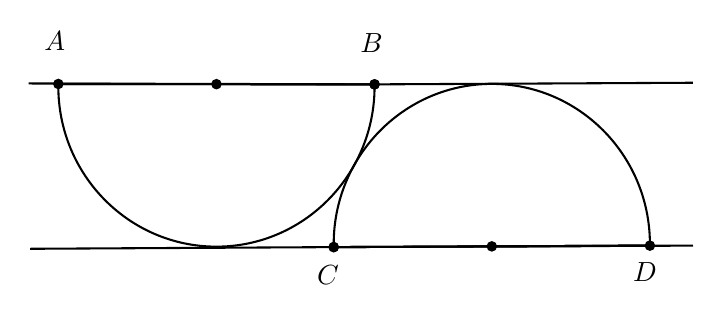
\begin{tikzpicture}[x=0.75pt,y=0.75pt,yscale=-1,xscale=1]
%uncomment if require: \path (0,513); %set diagram left start at 0, and has height of 513

%Shape: Chord [id:dp4346037350557095] 
\draw   (198.29,325.5) .. controls (198.3,325.86) and (198.3,326.23) .. (198.3,326.6) .. controls (198.25,369.22) and (164.11,403.73) .. (122.04,403.69) .. controls (79.97,403.64) and (45.9,369.06) .. (45.94,326.44) .. controls (45.94,326.06) and (45.95,325.69) .. (45.95,325.31) -- cycle ;
%Straight Lines [id:da2716887556237857] 
\draw    (351.67,324.72) -- (198.29,325.5) ;
\draw [shift={(198.29,325.5)}, rotate = 179.71] [color={rgb, 255:red, 0; green, 0; blue, 0 }  ][fill={rgb, 255:red, 0; green, 0; blue, 0 }  ][line width=0.75]      (0, 0) circle [x radius= 2.01, y radius= 2.01]   ;
%Straight Lines [id:da7916011663203262] 
\draw    (330.96,403.2) -- (178.62,403.91) ;
\draw [shift={(178.62,403.91)}, rotate = 179.73] [color={rgb, 255:red, 0; green, 0; blue, 0 }  ][fill={rgb, 255:red, 0; green, 0; blue, 0 }  ][line width=0.75]      (0, 0) circle [x radius= 2.01, y radius= 2.01]   ;
\draw [shift={(330.96,403.2)}, rotate = 179.73] [color={rgb, 255:red, 0; green, 0; blue, 0 }  ][fill={rgb, 255:red, 0; green, 0; blue, 0 }  ][line width=0.75]      (0, 0) circle [x radius= 2.01, y radius= 2.01]   ;
%Shape: Chord [id:dp6997928899051893] 
\draw   (178.62,403.91) .. controls (178.62,403.55) and (178.61,403.18) .. (178.61,402.81) .. controls (178.4,360.19) and (212.34,325.48) .. (254.41,325.27) .. controls (296.48,325.07) and (330.76,359.45) .. (330.96,402.07) .. controls (330.97,402.44) and (330.97,402.82) .. (330.96,403.2) -- cycle ;
%Straight Lines [id:da385160458787392] 
\draw    (178.62,403.91) -- (351.72,403.19) ;
%Straight Lines [id:da26518685481165716] 
\draw    (31.67,325.06) -- (198.29,325.5) ;
\draw [shift={(198.29,325.5)}, rotate = 0.15] [color={rgb, 255:red, 0; green, 0; blue, 0 }  ][fill={rgb, 255:red, 0; green, 0; blue, 0 }  ][line width=0.75]      (0, 0) circle [x radius= 2.01, y radius= 2.01]   ;
%Straight Lines [id:da9318274035877332] 
\draw    (32.33,404.72) -- (178.62,403.91) ;
\draw [shift={(178.62,403.91)}, rotate = 359.68] [color={rgb, 255:red, 0; green, 0; blue, 0 }  ][fill={rgb, 255:red, 0; green, 0; blue, 0 }  ][line width=0.75]      (0, 0) circle [x radius= 2.01, y radius= 2.01]   ;
%Straight Lines [id:da5888848958370978] 
\draw    (45.95,325.31) -- (198.29,325.5) ;
\draw [shift={(122.12,325.4)}, rotate = 0.07] [color={rgb, 255:red, 0; green, 0; blue, 0 }  ][fill={rgb, 255:red, 0; green, 0; blue, 0 }  ][line width=0.75]      (0, 0) circle [x radius= 2.01, y radius= 2.01]   ;
\draw [shift={(45.95,325.31)}, rotate = 0.07] [color={rgb, 255:red, 0; green, 0; blue, 0 }  ][fill={rgb, 255:red, 0; green, 0; blue, 0 }  ][line width=0.75]      (0, 0) circle [x radius= 2.01, y radius= 2.01]   ;
%Straight Lines [id:da18112325712169475] 
\draw    (254.79,403.56) -- (330.96,403.2) ;
\draw [shift={(254.79,403.56)}, rotate = 359.73] [color={rgb, 255:red, 0; green, 0; blue, 0 }  ][fill={rgb, 255:red, 0; green, 0; blue, 0 }  ][line width=0.75]      (0, 0) circle [x radius= 2.01, y radius= 2.01]   ;

% Text Node
\draw (37.67,298.69) node [anchor=north west][inner sep=0.75pt]    {$A$};
% Text Node
\draw (190,299.35) node [anchor=north west][inner sep=0.75pt]    {$B$};
% Text Node
\draw (169.17,411.52) node [anchor=north west][inner sep=0.75pt]    {$C$};
% Text Node
\draw (321.33,410.02) node [anchor=north west][inner sep=0.75pt]    {$D$};


\end{tikzpicture}
\end{center}
\end{problem}

\begin{problem} [\href{http://pmo.ph/wp-content/uploads/2018/08/PMO-Area-Stage-answers-only.pdf}{PMO 20 Areas I.7}]
Determine the area of the polygon formed by the ordered pairs $(x, y)$ where $x$ and $y$ are positive integers which satisfy the equation $$\dfrac{1}{x} + \dfrac{1}{y} = \dfrac{1}{13}.$$
\end{problem}



\section*{Solutions}

\vspace{3mm}

\begin{probboxed}[\href{http://pmo.ph/wp-content/uploads/2018/08/PMO-Area-Stage-answers-only.pdf}{PMO 20 Areas I.1}] Suppose that $x$ and $y$ are nonzero real numbers such that $\left(x + \dfrac{1}{y}\right)\left(y + \dfrac{1}{x}\right) = 7.$ Find the value of $\left(x^2 + \dfrac{1}{y^2}\right) \left(y^2 + \dfrac{1}{x^2}\right)$.

\end{probboxed}

\ans{25}

\sol We will expand the given expression:  $$\left(x + \dfrac{1}{y}\right)\left(y + \dfrac{1}{x}\right) = 7 \implies \left(xy + \dfrac{1}{xy} \right) = 5$$. Square the whole expression, this gives us 25. And notice that this is just equivalent to the value of the expression we are asked to find. Thus, the answer is \fbox{$25.$}


\begin{probboxed}[\href{https://pmo.ph/wp-content/uploads/2021/01/22nd-PMO-Area-Stage-with-solutions.pdf}{PMO 22 Areas I.1}]
If the sum of the first 22 terms of an arithmetic progression is 1045 and the sum of the next 22 terms is 2013, find the first term.

\end{probboxed}

\ans{$a_1 = \dfrac{53}{2}$}

\sol 

Let us see the problem in a mathematical notation: (In this case, let $a_1$ be the first term and $d$ be the common difference such that $a_n = a_1 + (n-1)d.$

\begin{equation*}
    \begin{array}{lll}
         \implies a_1 + (a_1 +d) + (a_1 +2d) + ... + (a_1 +21d) & = & 1045\\
         \\
         \implies (a_1 + 22d) + (a_1 + 23d) + (a_1 +24d) + ... + (a_1 +43d) & = & 2013\\
    \end{array}
\end{equation*}

Simplifying these equations we have:

\begin{equation*}
    \begin{array}{lll}
         \implies 22a_1 + 231d & = & 1045\\
         \\
         \implies 22a_1 + 715d & = & 2013\\
    \end{array}
\end{equation*}

Subtracting these two equations, notice that $22a_1$ cancels out. Because of this, we obtained $d= 2$. Substituting $d$ with 2 in the first equation, we have \fbox{$a_1 = \dfrac{53}{2}.$}

\newpage



\begin{probboxed}[\href{http://pmo.ph/wp-content/uploads/2018/08/PMO-Area-Stage-answers-only.pdf}{PMO 20 Areas I.3}]
Let $P$ be a point inside the isosceles trapezoid $ABCD$ where $AD$ is one of the bases, and let $P A, P B, P C$, and $P D$ bisect angles $A, B, C$, and $D$ respectively. If $PA=3$ and $\angle APD = 120 ^{\circ}$, find
the area of trapezoid $ABCD.$

\end{probboxed}

\ans{$6\sqrt{3}$}

\begin{rem}
The following figures that will be shown are not drawn to scale. 
\end{rem}

\sol

In every geometry problem, drawing the figure being described in the problem is very important. 
\begin{center}



\tikzset{every picture/.style={line width=0.75pt}} %set default line width to 0.75pt        

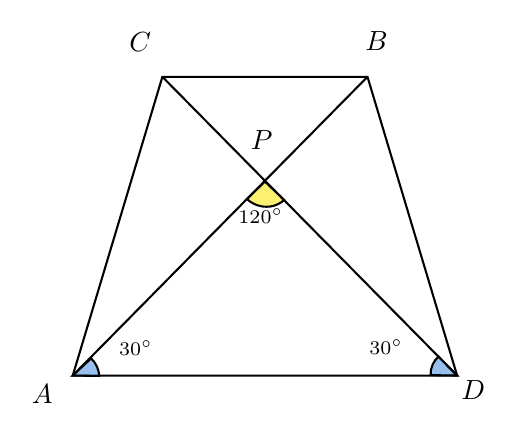
\begin{tikzpicture}[x=0.75pt,y=0.75pt,yscale=-1,xscale=1]
%uncomment if require: \path (0,300); %set diagram left start at 0, and has height of 300

%Shape: Trapezoid [id:dp458681184440368] 
\draw   (171,168.6) -- (214.18,24.67) -- (313,24.67) -- (356.18,168.6) -- cycle ;
%Straight Lines [id:da7632434328373614] 
\draw    (171,168.6) -- (313,24.67) ;
%Shape: Pie [id:dp8193547157796872] 
\draw  [fill={rgb, 255:red, 248; green, 231; blue, 28 }  ,fill opacity=0.63 ] (272.86,83.98) .. controls (269.31,87.35) and (263.67,88.34) .. (258.63,86.04) .. controls (257.22,85.4) and (255.98,84.56) .. (254.92,83.58) -- (263.58,75.13) -- cycle ;
%Straight Lines [id:da164820904825137] 
\draw    (356.18,168.6) -- (214.18,24.67) ;
%Shape: Pie [id:dp40952475405384914] 
\draw  [fill={rgb, 255:red, 74; green, 144; blue, 226 }  ,fill opacity=0.57 ] (179.85,160.33) .. controls (182.23,162.63) and (183.63,165.68) .. (183.76,168.79) -- (171,168.6) -- cycle ;
%Shape: Pie [id:dp09179526161598028] 
\draw  [fill={rgb, 255:red, 74; green, 144; blue, 226 }  ,fill opacity=0.57 ] (343.41,168.4) .. controls (343.34,166.67) and (343.65,164.91) .. (344.41,163.25) .. controls (345.08,161.78) and (346.04,160.51) .. (347.19,159.49) -- (356.18,168.6) -- cycle ;

% Text Node
\draw (249.33,86.67) node [anchor=north west][inner sep=0.75pt]  [font=\scriptsize]  {$120^{\circ }$};
% Text Node
\draw (255.28,49.03) node [anchor=north west][inner sep=0.75pt]    {$P$};
% Text Node
\draw (149.78,171.25) node [anchor=north west][inner sep=0.75pt]    {$A$};
% Text Node
\draw (356.78,169.75) node [anchor=north west][inner sep=0.75pt]    {$D$};
% Text Node
\draw (196.78,2) node [anchor=north west][inner sep=0.75pt]    {$C$};
% Text Node
\draw (310.53,1.5) node [anchor=north west][inner sep=0.75pt]    {$B$};
% Text Node
\draw (191.83,150.17) node [anchor=north west][inner sep=0.75pt]  [font=\scriptsize]  {$30^{\circ }$};
% Text Node
\draw (308.83,149.75) node [anchor=north west][inner sep=0.75pt]  [font=\scriptsize]  {$\ 30^{\circ }$};


\end{tikzpicture}
\end{center}

Since $\angle APD = 120^{\circ}$ and $AP$ and $PD$ are angle bisectors, then $\angle BAP = \angle PDC = \angle PAD = \angle PDA = 30^{\circ} $. Knowing the fact that if a trapezoid is isosceles, then its cyclic. Hence, $\angle ABC = \angle DCB = 120^{\circ}$. This implies that $\Delta APB$ is a 30-60-90 triangle and $BP = \sqrt{3}, AB = 2\sqrt{3}.$

\begin{center}
 


\tikzset{every picture/.style={line width=0.75pt}} %set default line width to 0.75pt        

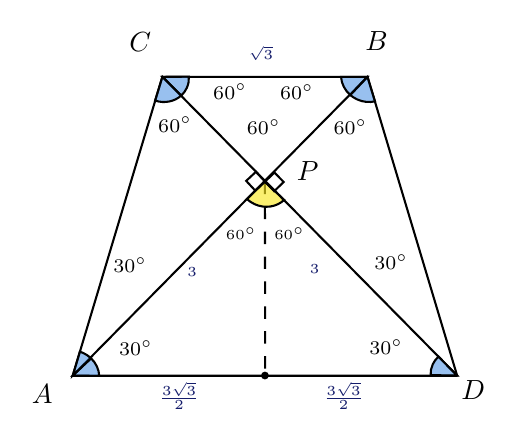
\begin{tikzpicture}[x=0.75pt,y=0.75pt,yscale=-1,xscale=1]
%uncomment if require: \path (0,300); %set diagram left start at 0, and has height of 300

%Straight Lines [id:da1153445473165513] 
\draw  [dash pattern={on 4.5pt off 4.5pt}]  (500.38,80.15) -- (500.5,173.5) ;
%Shape: Trapezoid [id:dp07564506452892639] 
\draw   (407.8,173.5) -- (450.98,29.57) -- (549.8,29.57) -- (592.98,173.5) -- cycle ;
%Straight Lines [id:da1524296869648567] 
\draw    (407.8,173.5) -- (549.8,29.57) ;
%Shape: Pie [id:dp9056637079944625] 
\draw  [fill={rgb, 255:red, 248; green, 231; blue, 28 }  ,fill opacity=0.63 ] (509.66,88.88) .. controls (506.11,92.25) and (500.47,93.24) .. (495.43,90.94) .. controls (494.02,90.3) and (492.78,89.46) .. (491.72,88.48) -- (500.38,80.03) -- cycle ;
%Straight Lines [id:da45323475676448277] 
\draw    (592.98,173.5) -- (450.98,29.57) ;
%Shape: Pie [id:dp7730589314484999] 
\draw  [fill={rgb, 255:red, 74; green, 144; blue, 226 }  ,fill opacity=0.57 ] (416.65,165.23) .. controls (419.03,167.53) and (420.43,170.58) .. (420.56,173.69) -- (407.8,173.5) -- cycle ;
%Shape: Pie [id:dp795879778624339] 
\draw  [fill={rgb, 255:red, 74; green, 144; blue, 226 }  ,fill opacity=0.57 ] (580.21,173.3) .. controls (580.14,171.57) and (580.45,169.81) .. (581.21,168.15) .. controls (581.88,166.68) and (582.84,165.41) .. (583.99,164.39) -- (592.98,173.5) -- cycle ;
%Shape: Pie [id:dp9408984897209249] 
\draw  [fill={rgb, 255:red, 74; green, 144; blue, 226 }  ,fill opacity=0.57 ] (463.73,29.51) .. controls (463.85,31.33) and (463.54,33.17) .. (462.75,34.91) .. controls (462.09,36.38) and (461.14,37.64) .. (459.99,38.66) -- (450.98,29.57) -- cycle ;
%Shape: Pie [id:dp7756274760317434] 
\draw  [fill={rgb, 255:red, 74; green, 144; blue, 226 }  ,fill opacity=0.57 ] (541.51,38.35) .. controls (538.86,36.05) and (537.26,32.88) .. (537.05,29.61) -- (549.8,29.57) -- cycle ;
%Shape: Pie [id:dp18897497795384743] 
\draw  [fill={rgb, 255:red, 74; green, 144; blue, 226 }  ,fill opacity=0.57 ] (460.06,38.6) .. controls (456.84,41.51) and (452.01,42.53) .. (447.46,41.04) -- (450.98,29.57) -- cycle ;
%Shape: Pie [id:dp05134607004311742] 
\draw  [fill={rgb, 255:red, 74; green, 144; blue, 226 }  ,fill opacity=0.57 ] (553.42,41.4) .. controls (550.69,42.02) and (547.67,41.76) .. (544.84,40.48) .. controls (543.6,39.91) and (542.48,39.19) .. (541.51,38.35) -- (549.8,29.57) -- cycle ;
%Shape: Pie [id:dp604426272247023] 
\draw  [fill={rgb, 255:red, 74; green, 144; blue, 226 }  ,fill opacity=0.57 ] (411.23,162) .. controls (411.74,162.16) and (412.25,162.36) .. (412.76,162.59) .. controls (414.18,163.24) and (415.44,164.09) .. (416.51,165.09) -- (407.8,173.5) -- cycle ;
%Shape: Square [id:dp004600651797676436] 
\draw   (491.36,79.72) -- (496.03,75.36) -- (500.38,80.03) -- (495.71,84.39) -- cycle ;
%Shape: Square [id:dp26332980319576915] 
\draw   (500.38,80.15) -- (504.94,75.68) -- (509.41,80.24) -- (504.85,84.7) -- cycle ;
%Straight Lines [id:da6467176939881425] 
\draw    (407.8,173.5) -- (592.98,173.5) ;
\draw [shift={(500.39,173.5)}, rotate = 360] [color={rgb, 255:red, 0; green, 0; blue, 0 }  ][fill={rgb, 255:red, 0; green, 0; blue, 0 }  ][line width=0.75]      (0, 0) circle [x radius= 1.34, y radius= 1.34]   ;

% Text Node
\draw (503.39,100.53) node [anchor=north west][inner sep=0.75pt]  [font=\tiny]  {$60^{\circ }$};
% Text Node
\draw (514.33,68.93) node [anchor=north west][inner sep=0.75pt]    {$P$};
% Text Node
\draw (386.58,176.15) node [anchor=north west][inner sep=0.75pt]    {$A$};
% Text Node
\draw (593.58,174.65) node [anchor=north west][inner sep=0.75pt]    {$D$};
% Text Node
\draw (433.58,6.9) node [anchor=north west][inner sep=0.75pt]    {$C$};
% Text Node
\draw (547.33,6.4) node [anchor=north west][inner sep=0.75pt]    {$B$};
% Text Node
\draw (428.63,155.07) node [anchor=north west][inner sep=0.75pt]  [font=\scriptsize]  {$30^{\circ }$};
% Text Node
\draw (545.63,154.65) node [anchor=north west][inner sep=0.75pt]  [font=\scriptsize]  {$\ 30^{\circ }$};
% Text Node
\draw (473.98,31.51) node [anchor=north west][inner sep=0.75pt]  [font=\scriptsize]  {$60^{\circ }$};
% Text Node
\draw (506.23,31.76) node [anchor=north west][inner sep=0.75pt]  [font=\scriptsize]  {$60^{\circ }$};
% Text Node
\draw (531.98,48.51) node [anchor=north west][inner sep=0.75pt]  [font=\scriptsize]  {$60^{\circ }$};
% Text Node
\draw (447.48,47.51) node [anchor=north west][inner sep=0.75pt]  [font=\scriptsize]  {$60^{\circ }$};
% Text Node
\draw (425.88,115) node [anchor=north west][inner sep=0.75pt]  [font=\scriptsize]  {$30^{\circ }$};
% Text Node
\draw (551.63,113.75) node [anchor=north west][inner sep=0.75pt]  [font=\scriptsize]  {$30^{\circ }$};
% Text Node
\draw (490.23,48.76) node [anchor=north west][inner sep=0.75pt]  [font=\scriptsize]  {$60^{\circ }$};
% Text Node
\draw (461.5,119.75) node [anchor=north west][inner sep=0.75pt]  [font=\tiny]  {$\textcolor[rgb]{0.08,0.11,0.42}{3}$};
% Text Node
\draw (520.5,118.5) node [anchor=north west][inner sep=0.75pt]  [font=\tiny]  {$\textcolor[rgb]{0.08,0.11,0.42}{3}$};
% Text Node
\draw (527,175.25) node [anchor=north west][inner sep=0.75pt]  [font=\tiny]  {$\textcolor[rgb]{0.08,0.11,0.42}{\frac{\textcolor[rgb]{0.08,0.11,0.42}{3\sqrt{3}}}{2}}$};
% Text Node
\draw (480.13,100.57) node [anchor=north west][inner sep=0.75pt]  [font=\tiny]  {$60^{\circ }$};
% Text Node
\draw (447.75,175.25) node [anchor=north west][inner sep=0.75pt]  [font=\tiny]  {$\textcolor[rgb]{0.08,0.11,0.42}{\frac{\textcolor[rgb]{0.08,0.11,0.42}{3}\textcolor[rgb]{0.08,0.11,0.42}{\sqrt{3}}}{2}}$};
% Text Node
\draw (491,13.25) node [anchor=north west][inner sep=0.75pt]  [font=\tiny]  {$\textcolor[rgb]{0.08,0.11,0.42}{\sqrt{3}}$};


\end{tikzpicture}
\end{center}

(Refer to the figure above): Since $\angle ACB = \angle ACD = \angle PBC = \angle ABP = 60$, and by angle chasing, $\angle BPC = 60$, then $\Delta BPC$ is equilateral. Now, we have the necessary information to find the area of the trapezoid, note that $AD = 3$. Hence, the altitude of $\Delta APD$ is $\frac{3}{2}$. Similarly, the altitude of $\Delta PBC$ is $\frac{3}{2}$. Note also that, the bases $AD$ and $BC$ are $3\sqrt{3}$ and $\sqrt{3}$, respectively. Hence, the area of the trapezoid is \fbox{$6\sqrt{3}$}.


\begin{probboxed}[\href{http://pmo.ph/wp-content/uploads/2018/08/PMO-Area-Stage-answers-only.pdf}{PMO 20 Areas I.5}] Let $f(x) = \sqrt{4\sin^4 x - \sin^2 x \cos^2 x + 4\cos^4 x }$ for any $x \in \mathbb{R}$. Let $M$ and $m$ be the maximum and minimum values of $f$, respectively. Find $Mm$.
\end{probboxed}

\ans{$\sqrt{7}$}
\sol

Let us rewrite the following expression in this fashion: 

\begin{equation*}
    \begin{array}{lll}
       \implies & f(x) = \sqrt{4\sin^4 x - \sin^2 x \cos^2 x + 4\cos^4 x }  & \\
         
         \\
         
         \implies & f(x) = \sqrt{4\left(\left(\sin^2 x + \cos^2 x\right)^2 - 2\sin^2 x \cos^2 \right) - \sin^2 x \cos^2 x}  \\
         
         \\
         
         \implies & f(x) = \sqrt{4 - 9\sin^2 x \cos^2x}  \\
         
         \\
         
        \implies & f(x) = \sqrt{4 - \dfrac{9(\sin^2 2x)}{4}}  \\ 
    \end{array}
\end{equation*}

Note that $0 \leq \sin^2 2x \leq 1$. This implies $M = \sqrt{4}$ and $m = \sqrt{\dfrac{7}{4}}$. Therefore, \fbox{$Mm = \sqrt{7.}$}



\begin{probboxed}
[\href{http://pmo.ph/wp-content/uploads/2020/12/18th-PMO-Area-Stage-Questions-and-Answers.pdf}{PMO 20 Areas I.9}] Two semicircles, each with radius $\sqrt{2}$, are tangent to each other, as shown in the figure below. If
$AB \hspace{2mm} || \hspace{2mm} CD$, determine the length of segment $AD$.

\begin{center}



\tikzset{every picture/.style={line width=0.75pt}} %set default line width to 0.75pt        

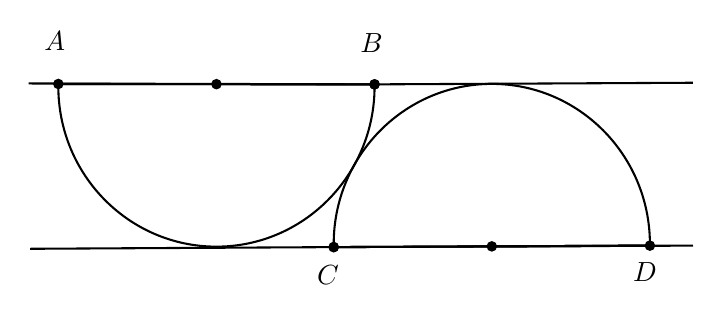
\begin{tikzpicture}[x=0.75pt,y=0.75pt,yscale=-1,xscale=1]
%uncomment if require: \path (0,513); %set diagram left start at 0, and has height of 513

%Shape: Chord [id:dp4346037350557095] 
\draw   (198.29,325.5) .. controls (198.3,325.86) and (198.3,326.23) .. (198.3,326.6) .. controls (198.25,369.22) and (164.11,403.73) .. (122.04,403.69) .. controls (79.97,403.64) and (45.9,369.06) .. (45.94,326.44) .. controls (45.94,326.06) and (45.95,325.69) .. (45.95,325.31) -- cycle ;
%Straight Lines [id:da2716887556237857] 
\draw    (351.67,324.72) -- (198.29,325.5) ;
\draw [shift={(198.29,325.5)}, rotate = 179.71] [color={rgb, 255:red, 0; green, 0; blue, 0 }  ][fill={rgb, 255:red, 0; green, 0; blue, 0 }  ][line width=0.75]      (0, 0) circle [x radius= 2.01, y radius= 2.01]   ;
%Straight Lines [id:da7916011663203262] 
\draw    (330.96,403.2) -- (178.62,403.91) ;
\draw [shift={(178.62,403.91)}, rotate = 179.73] [color={rgb, 255:red, 0; green, 0; blue, 0 }  ][fill={rgb, 255:red, 0; green, 0; blue, 0 }  ][line width=0.75]      (0, 0) circle [x radius= 2.01, y radius= 2.01]   ;
\draw [shift={(330.96,403.2)}, rotate = 179.73] [color={rgb, 255:red, 0; green, 0; blue, 0 }  ][fill={rgb, 255:red, 0; green, 0; blue, 0 }  ][line width=0.75]      (0, 0) circle [x radius= 2.01, y radius= 2.01]   ;
%Shape: Chord [id:dp6997928899051893] 
\draw   (178.62,403.91) .. controls (178.62,403.55) and (178.61,403.18) .. (178.61,402.81) .. controls (178.4,360.19) and (212.34,325.48) .. (254.41,325.27) .. controls (296.48,325.07) and (330.76,359.45) .. (330.96,402.07) .. controls (330.97,402.44) and (330.97,402.82) .. (330.96,403.2) -- cycle ;
%Straight Lines [id:da385160458787392] 
\draw    (178.62,403.91) -- (351.72,403.19) ;
%Straight Lines [id:da26518685481165716] 
\draw    (31.67,325.06) -- (198.29,325.5) ;
\draw [shift={(198.29,325.5)}, rotate = 0.15] [color={rgb, 255:red, 0; green, 0; blue, 0 }  ][fill={rgb, 255:red, 0; green, 0; blue, 0 }  ][line width=0.75]      (0, 0) circle [x radius= 2.01, y radius= 2.01]   ;
%Straight Lines [id:da9318274035877332] 
\draw    (32.33,404.72) -- (178.62,403.91) ;
\draw [shift={(178.62,403.91)}, rotate = 359.68] [color={rgb, 255:red, 0; green, 0; blue, 0 }  ][fill={rgb, 255:red, 0; green, 0; blue, 0 }  ][line width=0.75]      (0, 0) circle [x radius= 2.01, y radius= 2.01]   ;
%Straight Lines [id:da5888848958370978] 
\draw    (45.95,325.31) -- (198.29,325.5) ;
\draw [shift={(122.12,325.4)}, rotate = 0.07] [color={rgb, 255:red, 0; green, 0; blue, 0 }  ][fill={rgb, 255:red, 0; green, 0; blue, 0 }  ][line width=0.75]      (0, 0) circle [x radius= 2.01, y radius= 2.01]   ;
\draw [shift={(45.95,325.31)}, rotate = 0.07] [color={rgb, 255:red, 0; green, 0; blue, 0 }  ][fill={rgb, 255:red, 0; green, 0; blue, 0 }  ][line width=0.75]      (0, 0) circle [x radius= 2.01, y radius= 2.01]   ;
%Straight Lines [id:da18112325712169475] 
\draw    (254.79,403.56) -- (330.96,403.2) ;
\draw [shift={(254.79,403.56)}, rotate = 359.73] [color={rgb, 255:red, 0; green, 0; blue, 0 }  ][fill={rgb, 255:red, 0; green, 0; blue, 0 }  ][line width=0.75]      (0, 0) circle [x radius= 2.01, y radius= 2.01]   ;

% Text Node
\draw (37.67,298.69) node [anchor=north west][inner sep=0.75pt]    {$A$};
% Text Node
\draw (190,299.35) node [anchor=north west][inner sep=0.75pt]    {$B$};
% Text Node
\draw (169.17,411.52) node [anchor=north west][inner sep=0.75pt]    {$C$};
% Text Node
\draw (321.33,410.02) node [anchor=north west][inner sep=0.75pt]    {$D$};


\end{tikzpicture}
\end{center}
\end{probboxed}


\ans{$AD = 2\sqrt{3} + 2.$}

\sol First, find the length of $\omega ' \Lambda$.

\begin{center}
 


\tikzset{every picture/.style={line width=0.75pt}} %set default line width to 0.75pt        

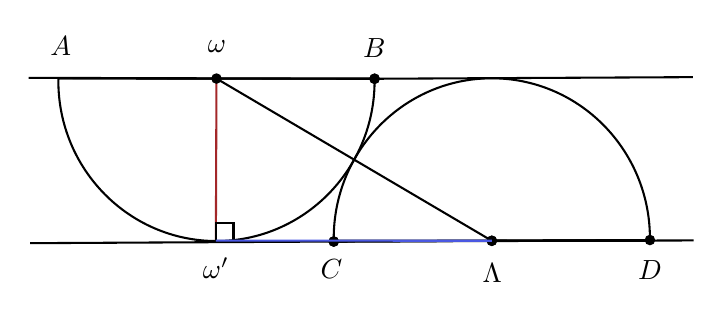
\begin{tikzpicture}[x=0.75pt,y=0.75pt,yscale=-1,xscale=1]
%uncomment if require: \path (0,513); %set diagram left start at 0, and has height of 513

%Shape: Chord [id:dp39163213637798977] 
\draw   (201.96,331.61) .. controls (201.96,331.97) and (201.97,332.34) .. (201.97,332.71) .. controls (201.92,375.33) and (167.78,409.84) .. (125.71,409.8) .. controls (83.63,409.75) and (49.56,375.17) .. (49.61,332.55) .. controls (49.61,332.17) and (49.61,331.8) .. (49.62,331.42) -- cycle ;
%Straight Lines [id:da4994200886527811] 
\draw    (355.33,330.83) -- (201.96,331.61) ;
\draw [shift={(201.96,331.61)}, rotate = 179.71] [color={rgb, 255:red, 0; green, 0; blue, 0 }  ][fill={rgb, 255:red, 0; green, 0; blue, 0 }  ][line width=0.75]      (0, 0) circle [x radius= 2.01, y radius= 2.01]   ;
%Straight Lines [id:da1592611313656529] 
\draw    (334.63,409.31) -- (182.29,410.03) ;
\draw [shift={(182.29,410.03)}, rotate = 179.73] [color={rgb, 255:red, 0; green, 0; blue, 0 }  ][fill={rgb, 255:red, 0; green, 0; blue, 0 }  ][line width=0.75]      (0, 0) circle [x radius= 2.01, y radius= 2.01]   ;
\draw [shift={(334.63,409.31)}, rotate = 179.73] [color={rgb, 255:red, 0; green, 0; blue, 0 }  ][fill={rgb, 255:red, 0; green, 0; blue, 0 }  ][line width=0.75]      (0, 0) circle [x radius= 2.01, y radius= 2.01]   ;
%Shape: Chord [id:dp599018789023438] 
\draw   (182.29,410.03) .. controls (182.28,409.66) and (182.28,409.29) .. (182.28,408.92) .. controls (182.07,366.3) and (216,331.59) .. (258.08,331.38) .. controls (300.15,331.18) and (334.42,365.56) .. (334.63,408.18) .. controls (334.63,408.56) and (334.63,408.93) .. (334.63,409.31) -- cycle ;
%Straight Lines [id:da33069645110800283] 
\draw    (182.29,410.03) -- (355.67,409.5) ;
%Straight Lines [id:da6474475154222319] 
\draw    (35.33,331.17) -- (201.96,331.61) ;
\draw [shift={(201.96,331.61)}, rotate = 0.15] [color={rgb, 255:red, 0; green, 0; blue, 0 }  ][fill={rgb, 255:red, 0; green, 0; blue, 0 }  ][line width=0.75]      (0, 0) circle [x radius= 2.01, y radius= 2.01]   ;
%Straight Lines [id:da5805793282183589] 
\draw    (36,410.83) -- (182.29,410.03) ;
\draw [shift={(182.29,410.03)}, rotate = 359.68] [color={rgb, 255:red, 0; green, 0; blue, 0 }  ][fill={rgb, 255:red, 0; green, 0; blue, 0 }  ][line width=0.75]      (0, 0) circle [x radius= 2.01, y radius= 2.01]   ;
%Straight Lines [id:da3124907607575145] 
\draw [color={rgb, 255:red, 163; green, 39; blue, 41 }  ,draw opacity=1 ]   (125.79,332.63) -- (125.5,409.58) ;
%Shape: Square [id:dp32951277611052054] 
\draw   (125.5,401.08) -- (134,401.08) -- (134,409.58) -- (125.5,409.58) -- cycle ;
%Straight Lines [id:da5500327654603556] 
\draw    (49.62,331.42) -- (201.96,331.61) ;
\draw [shift={(125.79,331.51)}, rotate = 0.07] [color={rgb, 255:red, 0; green, 0; blue, 0 }  ][fill={rgb, 255:red, 0; green, 0; blue, 0 }  ][line width=0.75]      (0, 0) circle [x radius= 2.01, y radius= 2.01]   ;
%Straight Lines [id:da1417171940338311] 
\draw    (182.29,409.57) -- (334.63,409.76) ;
\draw [shift={(258.46,409.67)}, rotate = 0.07] [color={rgb, 255:red, 0; green, 0; blue, 0 }  ][fill={rgb, 255:red, 0; green, 0; blue, 0 }  ][line width=0.75]      (0, 0) circle [x radius= 2.01, y radius= 2.01]   ;
%Straight Lines [id:da2274215904498651] 
\draw    (258.46,409.67) -- (334.63,409.31) ;
\draw [shift={(258.46,409.67)}, rotate = 359.73] [color={rgb, 255:red, 0; green, 0; blue, 0 }  ][fill={rgb, 255:red, 0; green, 0; blue, 0 }  ][line width=0.75]      (0, 0) circle [x radius= 2.01, y radius= 2.01]   ;
%Straight Lines [id:da07605749517178273] 
\draw    (125.79,331.51) -- (258.46,409.67) ;
%Straight Lines [id:da6174169333364647] 
\draw [color={rgb, 255:red, 74; green, 88; blue, 226 }  ,draw opacity=1 ]   (125.5,409.58) -- (258.46,409.67) ;

% Text Node
\draw (50.72,316) node    {$A$};
% Text Node
\draw (201.89,316.66) node    {$B$};
% Text Node
\draw (181.18,423.33) node    {$C$};
% Text Node
\draw (334.61,423.83) node    {$D$};
% Text Node
\draw (258.7,425.14) node    {$\Lambda $};
% Text Node
\draw (126.04,315.98) node    {$\omega $};
% Text Node
\draw (125.54,422.98) node    {$\omega '$};


\end{tikzpicture}
\end{center}

By Pythagorean theorem, $\omega ' \Lambda = \sqrt{\left(2\sqrt{2}\right)^2 - (\sqrt{2})^2} = \sqrt{6}.$ Finally, we can determine the length of $AD.$ By Pythagorean theorem again: $$AD^2 = 2 + \left(\sqrt{6} + 2\sqrt{2}\right)^2 = 16 + 8\sqrt{3}.$$ Hence, \fbox{$AD = 2\sqrt{3} + 2.$}

\begin{probboxed}[\href{http://pmo.ph/wp-content/uploads/2018/08/PMO-Area-Stage-answers-only.pdf}{PMO 20 Areas I.7}]

Determine the area of the polygon formed by the ordered pairs $(x, y)$ where $x$ and $y$ are positive integers which satisfy the equation $$\dfrac{1}{x} + \dfrac{1}{y} = \dfrac{1}{13}.$$

\end{probboxed}

\sol

Multiply both sides by $13xy$:

$$\dfrac{1}{x} + \dfrac{1}{y} = \dfrac{1}{13} \implies 13x + 13y - xy =0.$$

By Simon's Favorite Factoring Trick, $$(x-13)(y-13) = 169.$$ Finding $(x,y)$ such that $x,y$ are positive integers, we have $(26,26), (182,14), (14, 182)$. 

Now, we got the necessary information to find the area bounded by these coordinates. By shoelace theorem, we have: $$ \dfrac{1}{2} \big \lfloor \left(14\cdot26 + 26\cdot14 + 182^2 \right) - \left(14^2 + 182\cdot26 + 26\cdot182 \right) \big \rfloor& = & \fbox{12096}$$

\vspace{-1cm}

\begin{center}

\includegraphics[width=2.5in]{JOSH ROBERT OBAOB (2).png}
\end{center}



\end{document}
